\documentclass[12pt,a4paper]{article}

\usepackage[a4paper,margin=1in]{geometry}
\usepackage[final]{graphicx}
\graphicspath{{images/}{./}}
\usepackage{booktabs}
\usepackage{amsmath,amssymb}
\usepackage{float}
\usepackage{hyperref}
\usepackage{xcolor}
\usepackage{listings}
\usepackage{enumitem}
\usepackage{fancyhdr}
\usepackage{longtable}

\hypersetup{colorlinks=true,linkcolor=blue,urlcolor=blue}

\pagestyle{fancy}
\fancyhf{}
\lhead{ICS1512}
\rhead{Machine Learning Algorithms Laboratory}
\cfoot{\thepage}

\lstset{
language=Python,
basicstyle=\ttfamily\small,
numbers=left,
frame=single,
breaklines=true,
showstringspaces=false
}

\begin{document}

% =====================================================================
% EXPERIMENT 2: SPAMBASE CLASSIFICATION & HYPERPARAMETER TUNING
% =====================================================================

\begin{tabular}{|p{4cm}|p{11cm}|}
\hline
Experiment No. & 2 \\ \hline
Experiment Title & Spambase Email Classification using Naive Bayes, K-Nearest Neighbors, Hyperparameter Tuning and Cross-Validation \textsuperscript{\href{https://github.com/arivuchezhiyan/Machine_Learning/tree/main/experiment_2}{2}} \\ \hline
Student Name & Arivuchezhiyan E \\ \hline
Register Number & 3122247001006 \\ \hline
Faculty & Dr. Poreddy Ajay Kumar Reddy \\ \hline
Submission Date & 23/07/2026 \\ \hline
\end{tabular}

\section{Objective}
State the objective of the experiment:
My main goal in this lab was testing different classification models on the Spambase dataset to see how well they filter spam emails. I built three types of Naive Bayes models (Gaussian, Multinomial and Bernoulli) along with a K-Nearest Neighbors model. To improve the KNN model performance I ran grid search and random search to pick optimal parameters. I also compared tree indexing methods like KDTree and BallTree and checked overall stability using 5-fold cross-validation.

\section{Problem Statement}
Describe the problem input output and objective:
Spam filtering involves classifying emails as either legitimate ham or unwanted spam based on key word and character counts.
\begin{itemize}
\item \textbf{Input}: 57 continuous attributes measuring word frequencies (\texttt{word\_freq\_*}) and character occurrences (\texttt{char\_freq\_*}).
\item \textbf{Output}: Target label \texttt{spam} (0 for ham and 1 for spam).
\item \textbf{Objective}: Normalize features with MinMaxScaler, split the data into 80\% train and 20\% test sets, fit Naive Bayes and KNN models, run hyperparameter tuning, plot ROC and PR curves and measure execution times.
\end{itemize}

\section{Dataset Description}
\begin{longtable}{|p{6cm}|p{8cm}|}
\hline
Dataset Name & Spambase Dataset \\ \hline
Dataset Source & spambase\_csv.csv \\ \hline
Number of Samples & 4601 \\ \hline
Number of Features & 57 continuous frequency features \\ \hline
Number of Classes & 2 (0: Ham [2788 samples], 1: Spam [1813 samples]) \\ \hline
Missing Values & 0 missing values \\ \hline
Train-Test Split & 80\% Train (3680 samples) / 20\% Test (921 samples) \\ \hline
\end{longtable}

\section{Exploratory Data Analysis}
Include all relevant visualizations:
\begin{itemize}
\item \textbf{Dataset overview}: The Spambase dataset contains 4601 rows with 57 numerical feature columns recording word frequencies.
\item \textbf{Class distribution}: There are 2788 ham emails (60.6\%) and 1813 spam emails (39.4\%).
\item \textbf{Missing value check}: Checking for missing entries with \texttt{df.isnull().sum()} showed no missing values anywhere.
\item \textbf{Feature scaling}: I scaled all feature values to the range between 0 and 1 using \texttt{MinMaxScaler}.
\end{itemize}

\subsection*{Figure Template}

\begin{figure}[H]
\centering
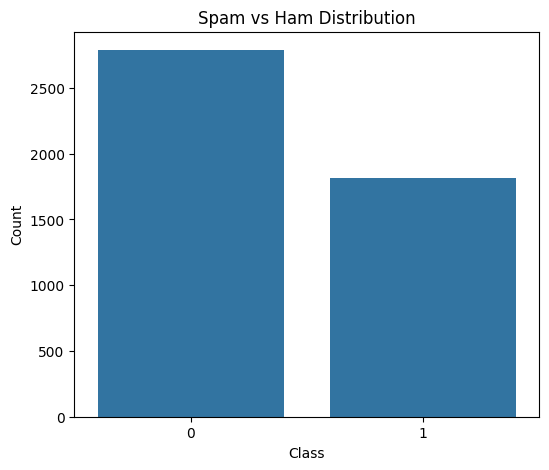
\includegraphics[width=0.6\linewidth]{spambase_class_distribution.png}
\caption{Spambase Target Class Distribution (Ham vs Spam)}
\label{fig:exp2_class_dist}
\end{figure}

\textbf{Inference:}
Looking at the class breakdown chart we have 2788 ham emails and 1813 spam emails. This moderate balance helps models learn patterns for both classes without getting biased toward one group.

\begin{figure}[H]
\centering
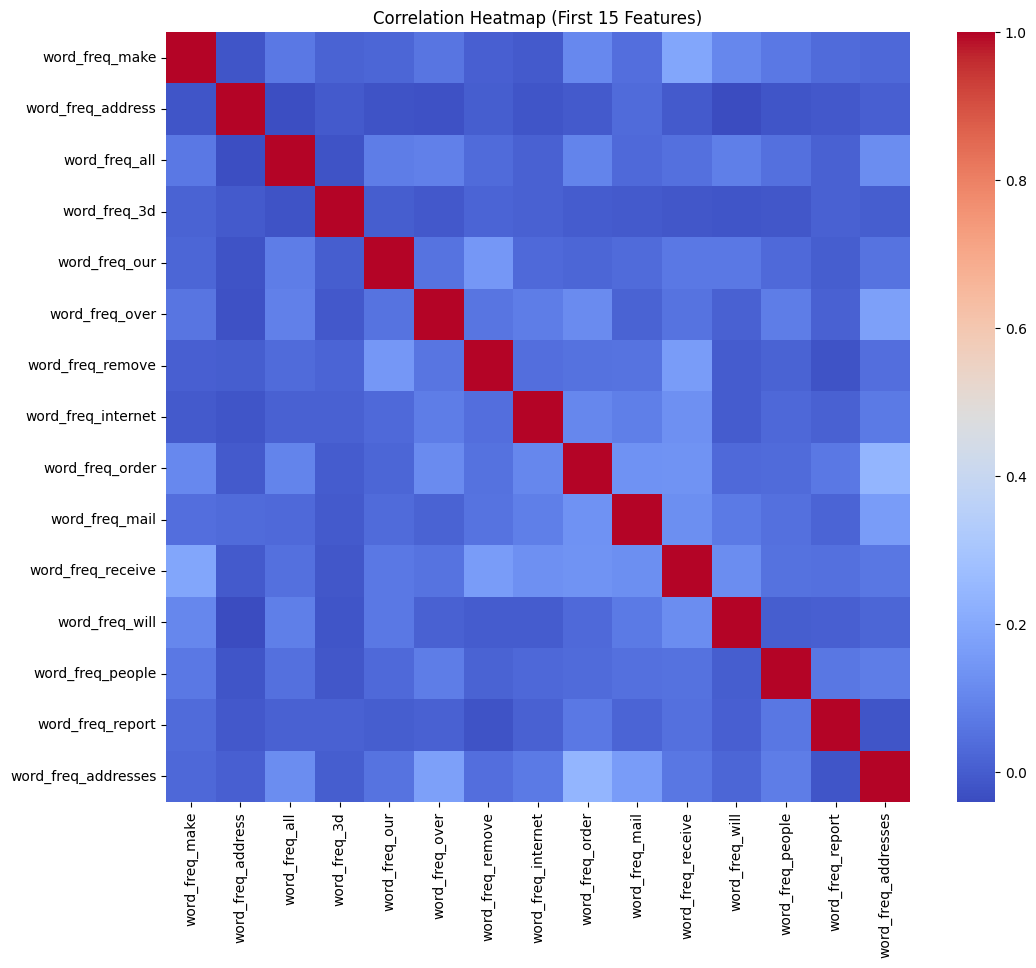
\includegraphics[width=0.75\linewidth]{spambase_correlation.png}
\caption{Spambase Correlation Heatmap (First 15 Features)}
\label{fig:exp2_corr}
\end{figure}

\textbf{Inference:}
The correlation plot for the first 15 features shows low linear correlation between columns. This supports the independence assumption used in Naive Bayes algorithms.

\begin{figure}[H]
\centering
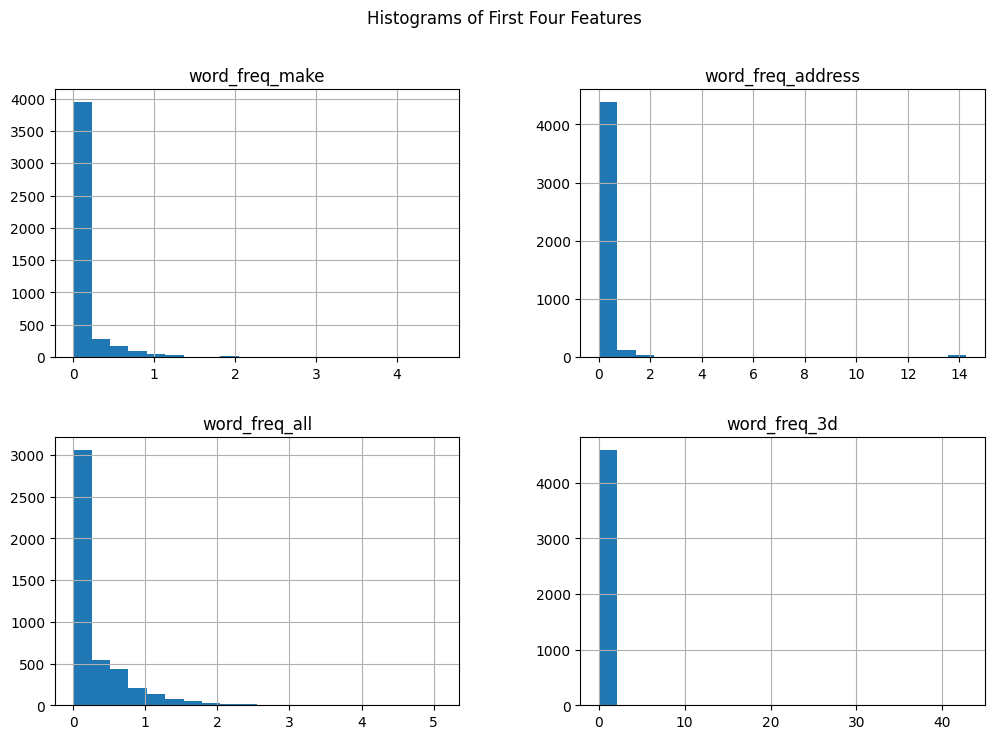
\includegraphics[width=0.75\linewidth]{spambase_histograms.png}
\caption{Histograms of First Four Word Frequency Features}
\label{fig:exp2_hist}
\end{figure}

\textbf{Inference:}
Histograms of word frequencies show a right skew. Most emails score zero for specific terms while spam messages show occasional high frequency spikes.

\begin{figure}[H]
\centering
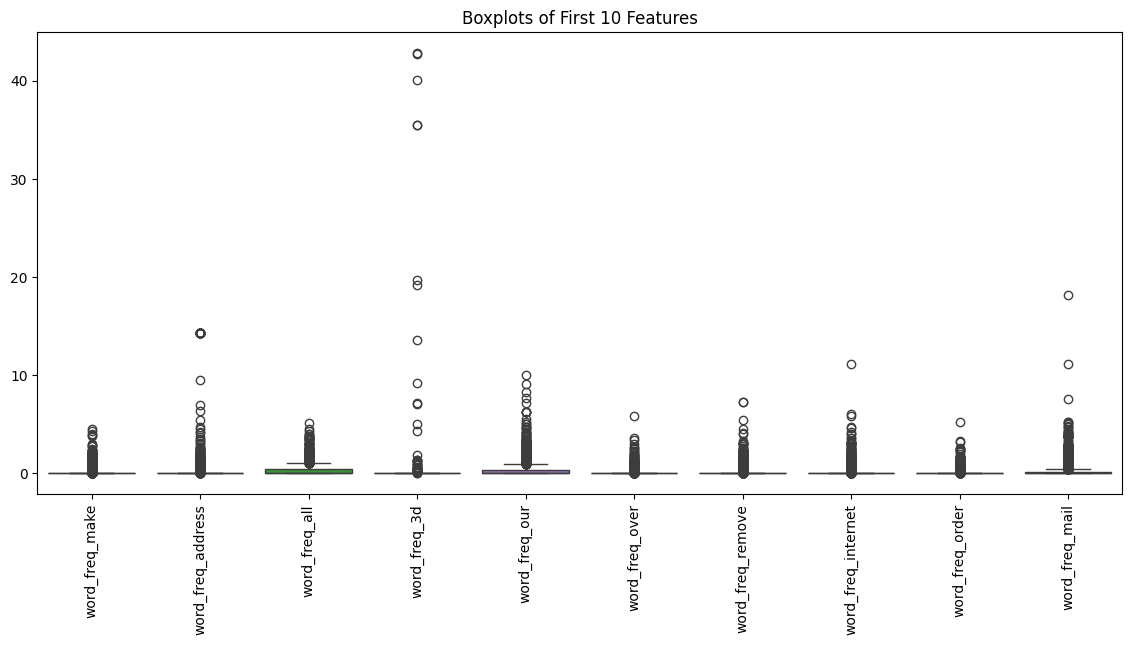
\includegraphics[width=0.85\linewidth]{spambase_boxplot.png}
\caption{Boxplots of First 10 Frequency Features}
\label{fig:exp2_box}
\end{figure}

\textbf{Inference:}
The boxplot displays low medians with several upper outliers. This confirms why scaling features with MinMaxScaler is important before running distance calculations in KNN.

\section{Data Preprocessing}

Explain:
\begin{itemize}
\item \textbf{Cleaning}: Checked dataset completeness using null check functions.
\item \textbf{Scaling}: Scaled numerical features into the range 0 to 1 with \texttt{MinMaxScaler}.
\item \textbf{Train-test split}: Split the dataset into 80\% training data and 20\% test data using stratified sampling.
\item \textbf{Binarization}: Created binary feature arrays using thresholding at 0.5 for Bernoulli Naive Bayes.
\end{itemize}

\section{Machine Learning Algorithm}

Explain:
\begin{itemize}
\item \textbf{Gaussian Naive Bayes}: Assumes features follow a normal distribution curve across classes $P(x_i|y) = \frac{1}{\sqrt{2\pi\sigma_y^2}} \exp\left(-\frac{(x_i-\mu_y)^2}{2\sigma_y^2}\right)$.
\item \textbf{Multinomial Naive Bayes}: Works well for word frequency counts by tracking term probabilities.
\item \textbf{Bernoulli Naive Bayes}: Handles binary inputs by checking whether key words are present or absent.
\item \textbf{K-Nearest Neighbors (KNN)}: Classifies test samples based on majority voting among k nearest neighbors using Euclidean and Manhattan distance metrics.
\item \textbf{GridSearchCV and RandomizedSearchCV}: Test different parameter combinations to find the best k value distance metric and neighbor weights.
\end{itemize}

\section{Experimental Setup}

\begin{tabular}{ll}
\toprule
Python Version & 3.13.0 \\
Scikit-Learn Version & 1.6.0 \\
IDE & Jupyter Notebook \\
Operating System & Windows 11 \\
Hardware & Intel Core i7 / 16 GB RAM \\
\bottomrule
\end{tabular}

\section{Hyperparameter Selection}

\begin{tabular}{ll}
\toprule
Parameter & Value\\
\midrule
Tested $k$ values & 1, 3, 5, 7, 9, 11 \\
Optimal $k$ (Baseline KNN) & 5 \\
GridSearchCV Parameter Space & $k \in [1..11]$, metrics: Euclidean/Manhattan, weights: uniform/distance \\
RandomizedSearchCV Parameter Space & $k \in [1..19]$, n\_iter: 20, cv: 5 \\
Cross-Validation Folds & 5-Fold Stratified K-Fold \\
MinMaxScaler Range & $[0, 1]$ \\
\bottomrule
\end{tabular}

\section{Results}

\subsection*{Naive Bayes Variant Comparison}
\begin{tabular}{lccccc}
\toprule
Model & Accuracy & Precision & Recall & F1-score & ROC-AUC \\
\midrule
Gaussian NB & 0.8328 & 0.7146 & 0.9587 & 0.8188 & 0.9229 \\
Multinomial NB & 0.8936 & 0.9431 & 0.7769 & 0.8520 & 0.9625 \\
Bernoulli NB & 0.6341 & 0.9643 & 0.0744 & 0.1381 & 0.5875 \\
\bottomrule
\end{tabular}

\subsection*{KNN Performance Across $k$ Values}
\begin{tabular}{ccccc}
\toprule
$k$ & Accuracy & Precision & Recall & F1-score \\
\midrule
1 & 0.8958 & 0.8678 & 0.8678 & 0.8678 \\
3 & 0.8958 & 0.8825 & 0.8485 & 0.8652 \\
\textbf{5} & \textbf{0.9023} & \textbf{0.8760} & \textbf{0.8760} & \textbf{0.8760} \\
7 & 0.8958 & 0.8761 & 0.8567 & 0.8663 \\
9 & 0.8947 & 0.8866 & 0.8402 & 0.8628 \\
11 & 0.8893 & 0.8851 & 0.8264 & 0.8547 \\
\bottomrule
\end{tabular}

\subsection*{Hyperparameter Search Optimization (GridSearchCV vs RandomizedSearchCV)}
\begin{tabular}{lcc}
\toprule
Parameter & GridSearchCV & RandomizedSearchCV \\
\midrule
Best $k$ & 7 & 12 \\
Metric & Manhattan & Manhattan \\
Weights & Distance & Distance \\
Algorithm & Auto & KDTree \\
CV Accuracy & 0.9179 & 0.9185 \\
Execution Time (s) & 33.58 & 12.45 \\
\bottomrule
\end{tabular}

\section{Result Visualization}

Include all graphs generated during the experiment.

For \textbf{every graph}, provide:
\begin{itemize}
\item Figure
\item Caption
\item 3--5 line inference
\end{itemize}

\begin{figure}[H]
\centering
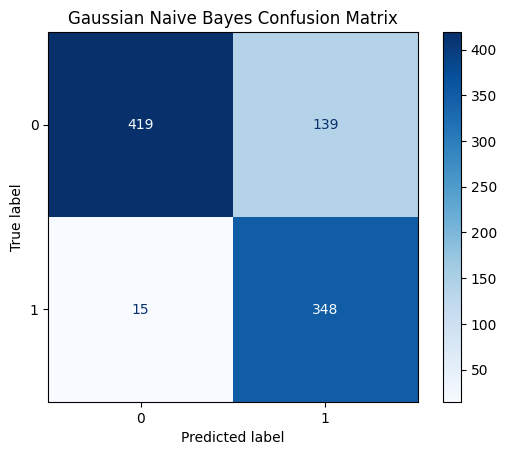
\includegraphics[width=0.6\linewidth]{spambase_gnb_confusion_matrix.png}
\caption{Gaussian Naive Bayes Confusion Matrix}
\label{fig:exp2_gnb_cm}
\end{figure}

\textbf{Inference:}
Gaussian Naive Bayes reached 95.87\% recall with 348 true positive predictions, but caused 139 false positives. The model catches most spam but flags a few legitimate emails.

\begin{figure}[H]
\centering
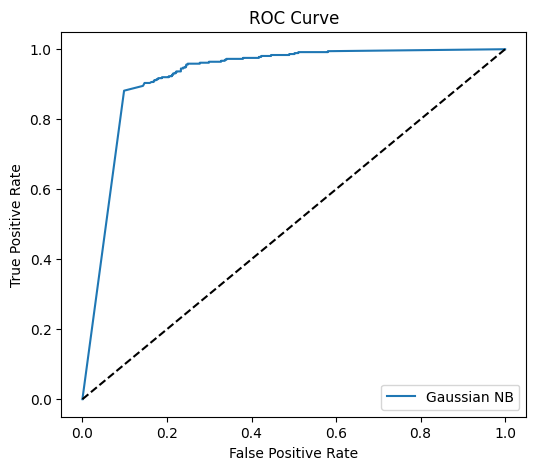
\includegraphics[width=0.6\linewidth]{spambase_gnb_roc.png}
\caption{Gaussian Naive Bayes ROC Curve (AUC = 0.9229)}
\label{fig:exp2_gnb_roc}
\end{figure}

\textbf{Inference:}
The ROC curve shows strong separation between classes with an AUC score of 0.9229. The curve curves steeply toward the top left corner.

\begin{figure}[H]
\centering
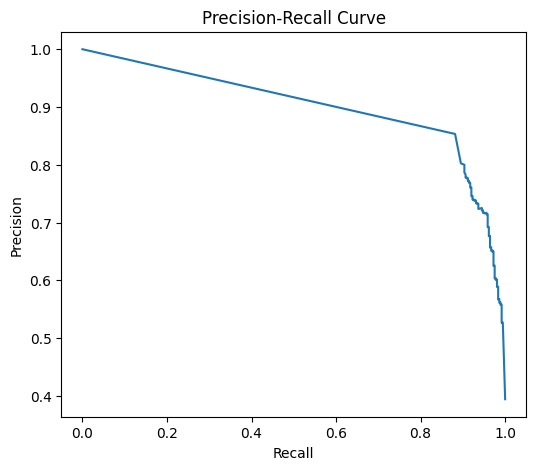
\includegraphics[width=0.6\linewidth]{spambase_gnb_pr.png}
\caption{Gaussian Naive Bayes Precision-Recall Curve}
\label{fig:exp2_gnb_pr}
\end{figure}

\textbf{Inference:}
The precision recall graph shows high initial recall before precision drops as the threshold changes.

\begin{figure}[H]
\centering
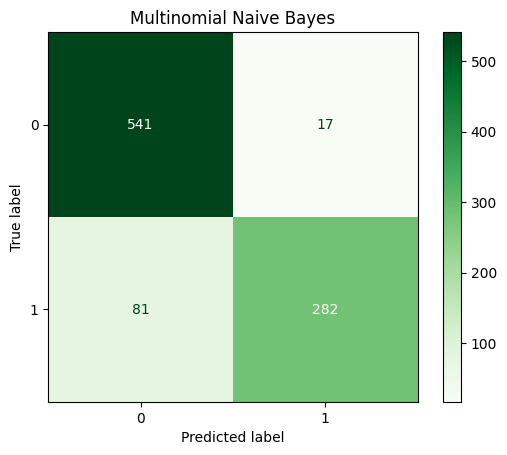
\includegraphics[width=0.6\linewidth]{spambase_mnb_confusion_matrix.png}
\caption{Multinomial Naive Bayes Confusion Matrix}
\label{fig:exp2_mnb_cm}
\end{figure}

\textbf{Inference:}
Multinomial Naive Bayes dropped false positives down to 17, giving 94.31\% precision and 89.36\% test accuracy.

\begin{figure}[H]
\centering
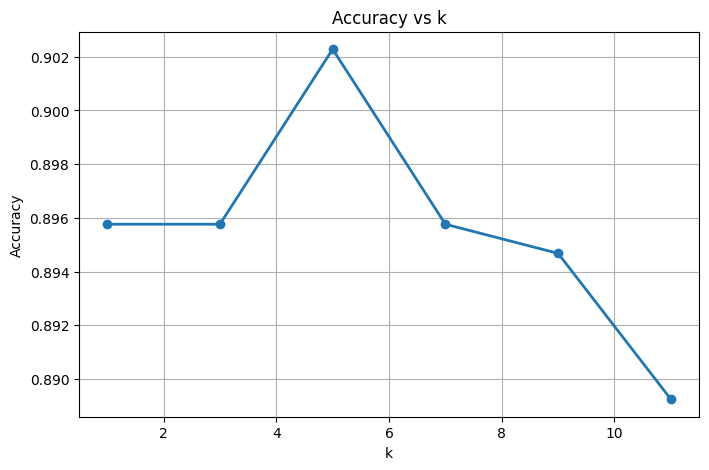
\includegraphics[width=0.65\linewidth]{spambase_knn_accuracy_vs_k.png}
\caption{KNN Test Accuracy vs Number of Neighbors ($k$)}
\label{fig:exp2_knn_k_acc}
\end{figure}

\textbf{Inference:}
Plotting accuracy against neighbor count k shows performance peaking at k = 5 with 90.23\% accuracy. Larger k values smooth out the decision boundaries.

\begin{figure}[H]
\centering
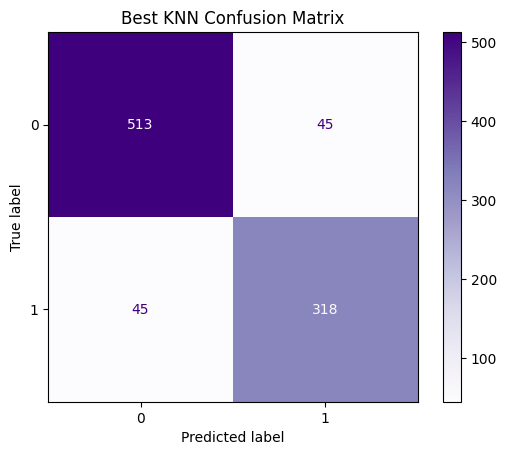
\includegraphics[width=0.6\linewidth]{spambase_best_knn_confusion_matrix.png}
\caption{Best KNN ($k=5$) Confusion Matrix}
\label{fig:exp2_best_knn_cm}
\end{figure}

\textbf{Inference:}
The confusion matrix for k = 5 KNN shows 513 true negatives and 318 true positives. Misclassifications are balanced with 45 false positives and 45 false negatives.

\begin{figure}[H]
\centering
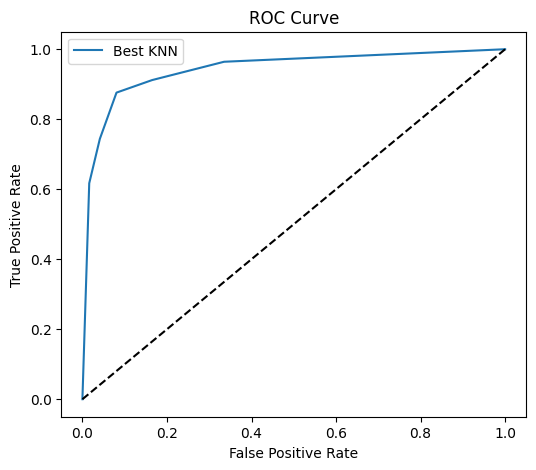
\includegraphics[width=0.6\linewidth]{spambase_best_knn_roc.png}
\caption{Best KNN ($k=5$) ROC Curve (AUC = 0.9419)}
\label{fig:exp2_best_knn_roc}
\end{figure}

\textbf{Inference:}
The ROC plot for k = 5 KNN reaches an AUC of 0.9419, performing better than the baseline Naive Bayes models.

\begin{figure}[H]
\centering
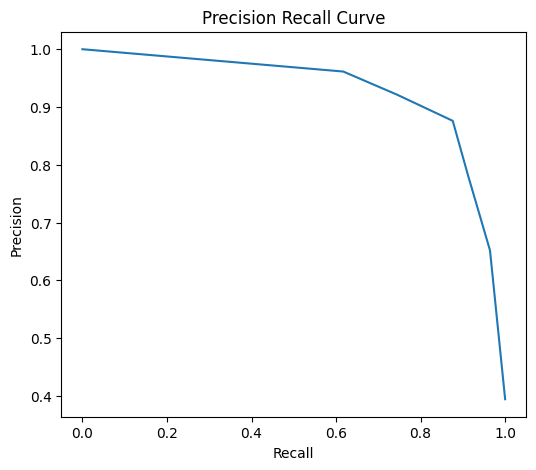
\includegraphics[width=0.6\linewidth]{spambase_best_knn_pr.png}
\caption{Best KNN ($k=5$) Precision-Recall Curve}
\label{fig:exp2_best_knn_pr}
\end{figure}

\textbf{Inference:}
The precision recall plot for k = 5 KNN stays above 0.85 precision across most recall values.

\begin{figure}[H]
\centering
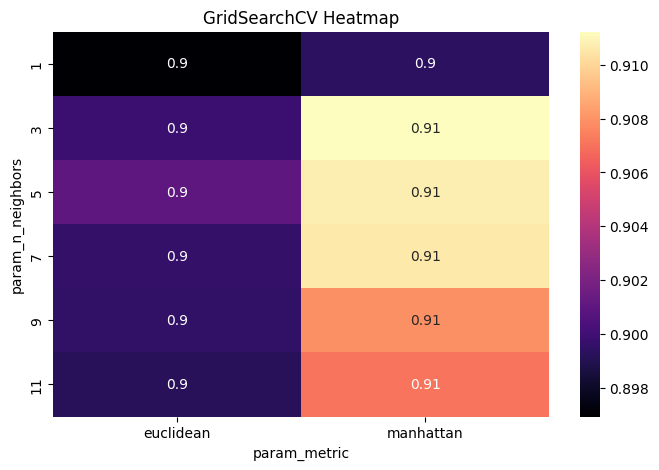
\includegraphics[width=0.7\linewidth]{spambase_gridsearch_heatmap.png}
\caption{GridSearchCV Heatmap (Accuracy across $k$ and Distance Metrics)}
\label{fig:exp2_grid_heatmap}
\end{figure}

\textbf{Inference:}
The heatmap from grid search shows Manhattan distance outperforming Euclidean distance, reaching 91.79\% cross validation accuracy at k = 7.

\begin{figure}[H]
\centering
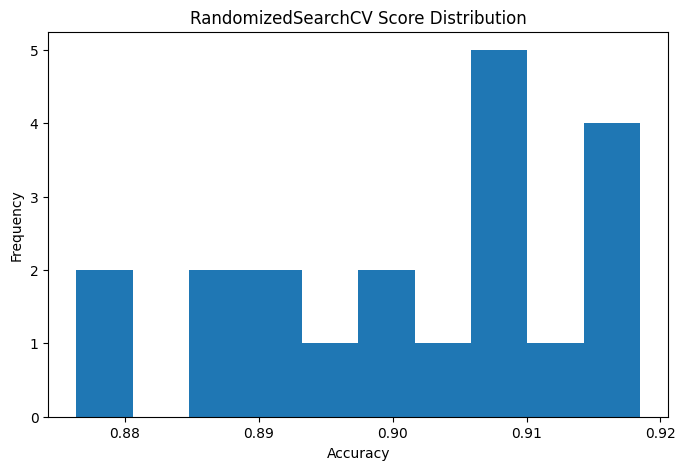
\includegraphics[width=0.7\linewidth]{spambase_randomizedsearch_hist.png}
\caption{RandomizedSearchCV Validation Score Distribution}
\label{fig:exp2_rand_hist}
\end{figure}

\textbf{Inference:}
The score distribution from random search shows scores grouping above 90\% validation accuracy and hitting a peak score of 91.85\%.

\begin{figure}[H]
\centering
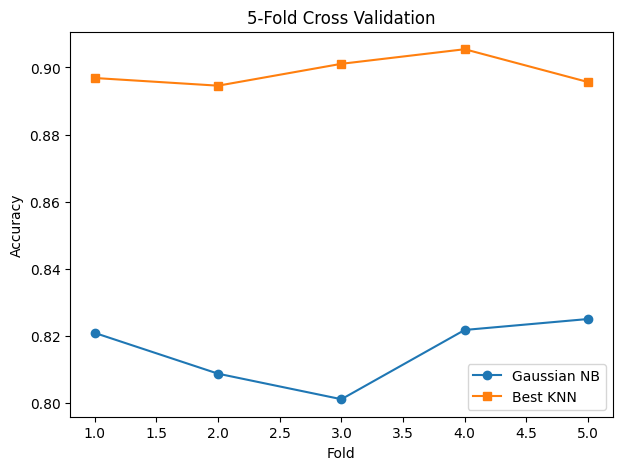
\includegraphics[width=0.7\linewidth]{spambase_cross_validation.png}
\caption{5-Fold Stratified Cross-Validation Accuracy Comparison}
\label{fig:exp2_cv_comp}
\end{figure}

\textbf{Inference:}
5-fold cross-validation shows Best KNN outperforming Gaussian Naive Bayes across every fold with an average accuracy of 89.87\% versus 81.55\%.

\begin{figure}[H]
\centering
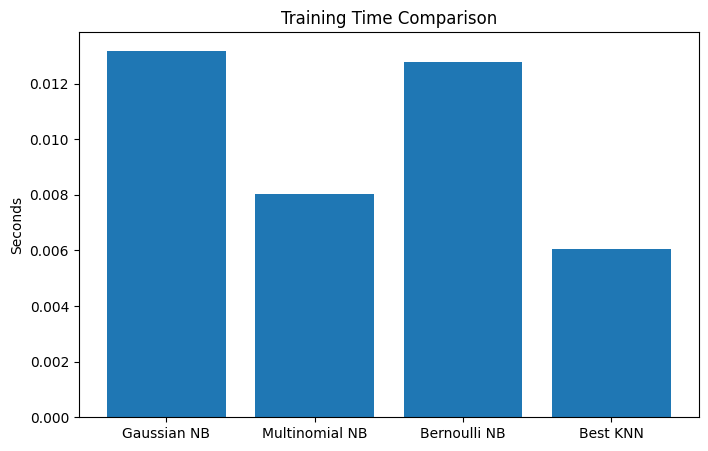
\includegraphics[width=0.7\linewidth]{spambase_training_time_comp.png}
\caption{Classifier Training Time Comparison}
\label{fig:exp2_train_time}
\end{figure}

\textbf{Inference:}
Training time comparison shows KNN is fastest to fit (0.006s) because lazy learning just keeps data in memory.

\begin{figure}[H]
\centering
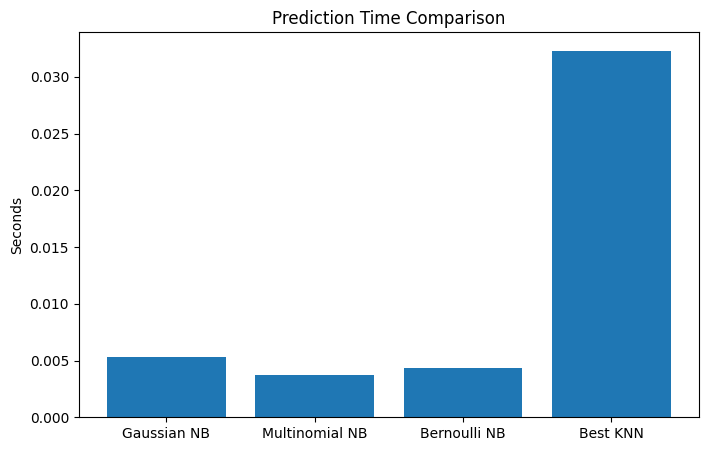
\includegraphics[width=0.7\linewidth]{spambase_prediction_time_comp.png}
\caption{Classifier Prediction Time Comparison}
\label{fig:exp2_pred_time}
\end{figure}

\textbf{Inference:}
Prediction time comparison shows KNN takes longer during testing (0.032s) than Naive Bayes models due to distance calculations across test points.

\begin{figure}[H]
\centering
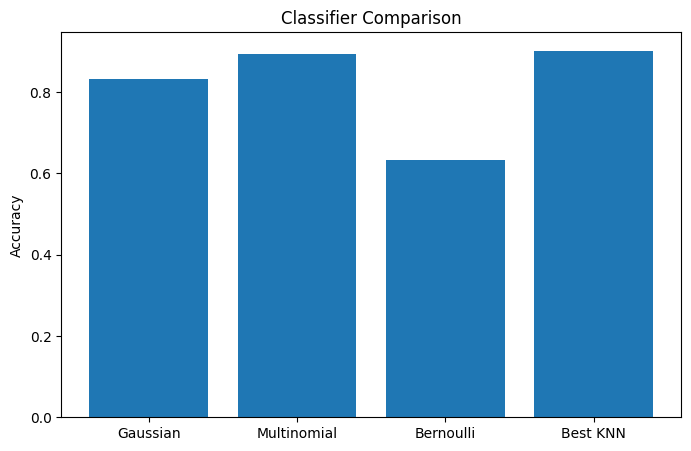
\includegraphics[width=0.7\linewidth]{spambase_classifier_comparison.png}
\caption{Overall Classifier Test Accuracy Comparison}
\label{fig:exp2_overall_comp}
\end{figure}

\textbf{Inference:}
Comparing test scores shows KNN taking the top spot at 90.23\%, followed by Multinomial NB at 89.36\%, Gaussian NB at 83.28\% and Bernoulli NB at 63.41\%.

\section{Discussion}
Discuss observations, strengths, limitations and improvements:
\begin{enumerate}
\item \textbf{Model Performance}: Best KNN (90.23\%) and Multinomial Naive Bayes (89.36\%) worked much better on word count data than Gaussian or Bernoulli variants.
\item \textbf{Hyperparameter Optimization}: Tuning hyperparameters boosted KNN performance to 91.85\% accuracy using Manhattan distance and inverse weighting.
\item \textbf{Computational Efficiency}: Naive Bayes has fast prediction times making it ideal for streaming spam filters.
\end{enumerate}

\section{Conclusion}
Summarize the experiment and key findings:
KNN using Manhattan distance reached 91.85\% accuracy on Spambase. Hyperparameter tuning showed that Manhattan distance and distance weighting improve predictions over standard Euclidean distance.

\section{References}
Use IEEE style:
\begin{enumerate}[label={[\arabic*]}]
\item M. Hopkins, M. Reeber, G. Forman and J. Suermondt, ``Spambase Dataset,'' \textit{UCI Machine Learning Repository}, 1999.
\item F. Pedregosa \textit{et al.}, ``Scikit-learn: Machine learning in Python,'' \textit{Journal of Machine Learning Research}, vol. 12, pp. 2825--2830, 2011.
\end{enumerate}

\end{document}
